\documentclass[11pt, english]{article}
\usepackage[svgnames]{xcolor}
\usepackage{booktabs}
\usepackage{graphicx}
\usepackage[flushleft]{threeparttable}
\usepackage[colorlinks=true, linkcolor=blue]{hyperref}
\usepackage{float}
\usepackage[utf8]{inputenc}
\usepackage[T1]{fontenc}
\usepackage[utf8]{inputenc}
\usepackage{listingsutf8}
\usepackage[spanish]{babel}
\selectlanguage{spanish}
\usepackage{amsmath}


\usepackage{listings}
\usepackage{afterpage}

\pagestyle{plain}

\definecolor{dkgreen}{rgb}{0,0.6,0}
\definecolor{gray}{rgb}{0.5,0.5,0.5}
\definecolor{mauve}{rgb}{0.58,0,0.82}
%\lstset{language=R,
%    basicstyle=\small\ttfamily,
%   stringstyle=\color{DarkGreen},
%    otherkeywords={0,1,2,3,4,5,6,7,8,9},
%    morekeywords={TRUE,FALSE},
%    deletekeywords={data,frame,length,as,character},
%    keywordstyle=\color{blue},
%    commentstyle=\color{DarkGreen},
%}

\lstset{frame=tb,
language=Java,
aboveskip=3mm,
belowskip=3mm,
showstringspaces=false,
columns=flexible,
numbers=none,
keywordstyle=\color{blue},
numberstyle=\tiny\color{gray},
commentstyle=\color{dkgreen},
stringstyle=\color{mauve},
breaklines=true,
breakatwhitespace=true,
tabsize=3,
inputencoding=utf8/latin1,
extendedchars=true,
literate={á}{{\'a}}1 {é}{{\'e}}1 {ó}{{\'o}}1 {ú}{{\'u}}1 {ü}{{\"u}}1 {ñ}{{\~n}}1 {¿}{{?`}}1 {¡}{{!`}}1
}

\usepackage{here}


\textheight=21cm
\textwidth=17cm
%\topmargin=-1cm
\oddsidemargin=0cm
\parindent=0mm
\pagestyle{plain}

%%%%%%%%%%%%%%%%%%%%%%%%%%
% La siguiente instrucción pone el curso automáticamente%
%%%%%%%%%%%%%%%%%%%%%%%%%%

\usepackage{color}
\usepackage{ragged2e}

\global\let\date\relax
\newcounter{unomenos}
\setcounter{unomenos}{\number\year}
\addtocounter{unomenos}{-1}
\stepcounter{unomenos}
\gdef\@date{ Curso  2018 / \arabic{unomenos}}

\begin{document}

\begin{titlepage}

\begin{center}
\vspace*{-1in}
\begin{figure}[htb]
\begin{center}
\includegraphics[width=10cm]{../res/pics/logo.jpg}
\end{center}
\end{figure}

\vspace*{0.4in}
\begin{large}
\textsc{Procesadores de Lenguaje}:\\
\end{large}
\vspace*{0.2in}
\begin{Large}
\textbf{\textsc{Nombre de nuestro lenguaje}} \\
\end{Large}
\vspace*{0.3in}
\begin{large}
\@date\\
\end{large}
\vspace*{0.3in}invalid utf-8 byte sequence spanish characters listing latex
\rule{80mm}{0.1mm}\\
\vspace*{0.1in}
\begin{large}
Realizado por: \\

Medina Medina, David Alberto  \\
Brito Ramos, Christian  \\
Hernández Delgado, Christopher \\
López González, Néstor \\
\vspace*{0.3in}
\end{large}

\includegraphics[width=3cm]{../res/pics/LogoEscuela.jpg}
\end{center}
\end{titlepage}

\newcommand{\CC}{C\nolinebreak\hspace{-.05em}\raisebox{.4ex}{\tiny\bf +}\nolinebreak\hspace{-.10em}\raisebox{.4ex}{\tiny\bf +}}
\def\CC{{C\nolinebreak[4]\hspace{-.05em}\raisebox{.4ex}{\tiny\bf ++}}}

\tableofcontents
\newpage

\section{Definición del lenguaje (Autor: Quien termine antes)}\label{Introduction}
Introducir breve introducción del lenguaje que planteamos.
\newpage

\subsection{Tipos de datos}\label{data-type}
Cualquier leguaje de programación necesita definir un conjunto de \emph{tipos de datos}, esto es, la batería de valores y operaciones que puede adquirir una variable. Cada tipo de dato está definido en el lenguaje por un \emph{literal} único que lo representa, lo que permite que cada tipo de dato tenga un representación física específica.

Los tipos de datos definidos en el lenguaje son los que figuran en el \emph{cuadro \ref{tab:table1}}. Las características críticas de implementación que define a cada tipo son:

\begin{description}
	\item[Entero] Representa a todas y cada una de las variables enteras que sean declaradas en el lenguaje. Este tipo de dato presenta un tamaño de 4 bytes (32 bits) y permite representar números enteros con signo. El \emph{complemento a 2} es el sistema elegido para definir el signo del número entero. Este dato se representa por el literal \texttt{int}. El rango de valores que puede tomar es

	\begin{equation}\label{eq:equation1}
		\left [-2^{N-1},\: 2^{N-1}-1 \right ] = \left [-2^{32-1},\: 2^{32-1}-1 \right] = \left [-2147483648,\: 2147483647 \right]
	\end{equation}

	donde, $N$ es el número de bits disponibles para representar el número entero (32 bits).
	\item[Coma flotante de simple precisión] Este tipo de dato representa número reales en coma flotante de simple precisión con un tamaño de 4 bytes (32 bits) siguiendo el estándar \emph{IEEE 754}. En la figura \ref{fig:figure1} puede observarse como esta representación binaria los bits se organizan en tres sectores principales:
	\begin{itemize}
		\item \textbf{Signo} (1 bit). Se trata de un sólo bit que define el signo del número: positivo (0) o negativo (1).
		\item  \textbf{Exponente (8bits)}. Se trata de un número entero con signo de complemento a 2 ($\left [ -128,\: 127\right ]$)
		\item \textbf{Mantisa (23 bits)}. Conforma la fracción a la derecha de la coma binaria y un bit de encabezado implícito.
	\end{itemize}
	Este tipo de dato se representa con el literal \texttt{real}. Su rango de valores es de $\left [ 1.18 \cdot 10^{–38},\; 3.4 \cdot 10^{38} \right ]$.
	\begin{figure}[H]\label{fig:figure1}
		\centering
		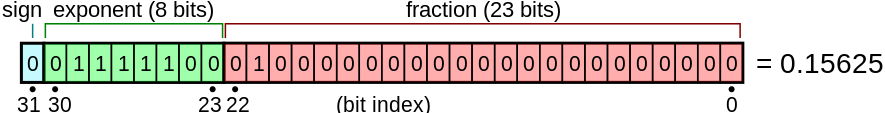
\includegraphics[width=0.75\textwidth]{../res/pics/data-types/float_diag.png}
		\caption{Representación binaria de número en coma flotante de simple precisión (\emph{IEEE 754})}
	\end{figure}

	\item[Caracter] Este tipo de dato es usado para representar caracteres con la codificación \emph{ASCII}, es por este motivo que el tamaño de que ocupan las variables de tipo caracter son de 1 byte de tamaño, siendo \texttt{char} el literal que lo representa.
	\item[Booleano] Se trata de un tipo de dato utilizado para representar representar valores booleanos. Su tamaño es de 1 bit, por lo que tan solo puede tomar dos valores: \texttt{1} (verdadero) ó \texttt{0} (falso). El literal que lo representa es \texttt{bool}.
\end{description}

\begin{table}[H]
	\begin{center}
		\caption{Tipos de datos}
		\label{tab:table1}
		\begin{tabular}{l|l|l|l|l}
			\toprule
			\textbf{Tipo} & \textbf{Literal} & \textbf{Patrón \texttt{REGEX}} & \textbf{Tamaño} & \textbf{Rango}\\
			\midrule
			Entero & int & ([0-9]+[\^.]) & 4 Bytes & $\left [-2147483648,\: 2147483647 \right]$\\
			Coma flotante de simple precisión & real & ([0-9]+[.][0-9]*) & 4 Byte & $\left [ 1.18 \cdot 10^{–38},\; 3.4 \cdot 10^{38} \right ]$\\
			Caracter & char & (['][\textbackslash W|\textbackslash w]?[']) & 1 Byte & $\left [ \texttt{0x00 - 0xFF} \right ]$\\
			Lógico & bool & (true|false)  & 1 Bit & $\left [0,\; 1 \right ]$\\
			\bottomrule
		\end{tabular}
	\end{center}
\end{table}

En el siguiente ejemplo se muestra cómo se declaran las variables con los literales de los tipos descritos anteriormente:

\lstinputlisting[language=C++]{../res/lst/data-types/data-type.x}

\subsection{Colecciones de datos: \texttt{Arrays}}\label{arrays}
Las variables pueden ser agrupadas en colecciones de datos de una dimensión denominados \texttt{arrays}. En este lenguaje, cualquier tipo de dato puede formar parte de un \texttt{array}.

Para declarar un \texttt{array} del tipo que se desee, debe usar la gramática \ref{grammar:1.2.1}:
	\begin{equation}\label{grammar:1.2.1}
		tipo[<int>]\; nombre\_variable
	\end{equation}

donde el $tipo$ define el tipo de dato e $<int>$ un valor entero opcional que define el tamaño del \texttt{array}. Cuando no se indica este último valor entero, no se lleva a término la reserva en memoria del \texttt{array} declarado. En caso contrario, se reservará en memoria tantos bytes/bits como fueren necesarios para generar una colección de tipos de datos del tamaño indicado por $<int>$. El número de bytes/bits a reservar está determinado por el tipo de dato y el tamaño del \texttt{array},
	\begin{equation}\label{eq:1.2}
		Tamano_{memoria} = Tamano_{tipo\, dato} \times Tamano_{array}
	\end{equation}

Un \texttt{array} que ha sido declarado con anterioridad puede ser redefinido haciendo uso de la gramática \ref{grammar:1.2.2},
	\begin{equation}\label{grammar:1.2.2}
	tipo[ \, ]\; nombre\_variable = new\; tipo[<int>]\; \{ \\
	expresion\_1, expresion\_2, ...\;\}
	\end{equation}

Esta notación es alternativa a la gramática \ref{grammar:1.2.1}, donde podremos inicializar el \texttt{array} a un conjunto de expresiones separados por comas encerrados dentro de los caracteres \texttt{\{} y \texttt{\}}. Estas expresiones son opcionales. El tamaño máximo del vector y, por tanto, de expresiones es el indicado por $<int>$ el cual es un número entero de caracter obligatorio.

Si se declara un \texttt{array} utilizando la gramática \ref{grammar:1.2.1} o \ref{grammar:1.2.2} sin expresiones en esta última, el array es inicializado en todas sus posiciones al valor \texttt{0} para tipos de datos enteros y reales. Para caracteres el valor por defecto es el caracter \texttt{nulo}. Y para tipos booleanos el valor por defecto es \texttt{FALSE}.

La gramática \ref{grammar:1.2.3} es necesaria para acceder al valor de un elemento del \texttt{array} en una posición arbitraria del mismo,
	\begin{equation}\label{grammar:1.2.3}
	nombre\_variable\; [<int>]
	\end{equation}
donde $<int>$ es un entero obligatorio que indica la posición del \texttt{array} a la que se desea acceder.

El \texttt{array} de caracteres constituyen los denominados \texttt{string}, los cuales requieren una atención especial ya que es posible cargar una variable con una secuencia de caracteres sin ser necesaria la declaración dada por la gramática \ref{grammar:1.2.2}. La gramática \ref{grammar:1.2.4} define la instancia de un \texttt{string} con un conjunto de caracteres localizados entre los caracteres comillas doble,

	\begin{equation}\label{grammar:1.2.4}
	nombre\_variable\; = " <char><char>..."
	\end{equation}

El siguiente listado muestra algunos ejemplos de uso de los \texttt{array} definidos en este lenguaje:

\lstinputlisting[language=C++, caption=Ejemplo de uso de arrays]{../res/lst/array/array.x}

\subsection{Palabras reservadas y cambios de contexto}
Este lenguaje utiliza una serie de palabras reservadas que se utilizan para desempeñar las funciones aquí descritas:
\begin{description}
	\item[\texttt{continue}] La sentencia de continue es de tipo de control de bucles. Dentro de la iteracion en un bucle, de cualquiera de los tipos (while, do-while, for), el uso de esta sentencia rompe la iteracion de dicho bucle. Provocando que se ejecute la siguiente iteracion de dicho bucle, ignorando las sentencias posteriores a "continue".
	\item[\texttt{break}] Dentro de la iteracion en un bucle, de cualquiera de los tipos (while, do-while, for), el uso de esta sentencia rompe la iteracion de dicho bucle.
	\item[\texttt{return}] Palabra empleada para retornar el resultado de un método o función, además de interrumpir la ejecución del mismo.
	\item[\texttt{void}] Es utilizado para indicar que una función no debe devolver ningún valor.
	\item[\texttt{fun}] Palabra especial utilizada al principio de cada declaración o definición de funciones.
\end{description}

Los \textbf{cambios de contexto} de bloques de instrucciones son aplicables cuando se hace uso de un caracter \texttt{0x09} (\texttt{TAB}) o de 4 espacios consecutivos (\texttt{0x20}).

\subsection{Comentarios}
Aquí va el texto. Poner siempre un código de ejemplo.
\begin{itemize}
	\item \textbf{'Comentario de línea'} . Para indicar un comentario de línea, basta con comenzar con '..', siendo el resultado final '.. {TEXTO}'.
\begin{lstlisting}[caption=Ejemplo de comentario de línea]
int a = 7
.. Variable que almacena una suma.
int suma = 0
suma = 30 + a
\end{lstlisting}
	\item \textbf{'Comentario de bloque'} . Los comentarios de varias líneas se establecen utilizando ',.' y '.,'  quedando como resultado ',. {VARIAS LÍNEAS DE TEXTO} .,'.
\begin{lstlisting}[caption=Ejemplo de comentario de bloque]
int a = 7
int suma = 0
suma = 30 + a
,.
En este punto, la variable suma toma el
valor de 37.
.,
\end{lstlisting}
\end{itemize}

\subsection{Tipos de operadores}\label{operators}
El conjunto de posibles operadores aplicables a nuestro lenguaje pueden clasificarse en:
\begin{itemize}
	\item Operadores aritméticos
	\item Operadores lógicos
	\item Operadores bit a bit
	\item Operadores de array
\end{itemize}


\subsubsection{Operadores aritméticos}\label{arithmetic-operators}
Estos operadores son necesarios para realizar operaciones matemáticas sencillas. La descripción detallada de cada uno de estos operadores queda reflejado en la tabla \ref{tab:arithmetic}.

\begin{table}[H]
	\begin{center}
		\caption{Operadores aritméticos}\label{tab:arithmetic}
		\begin{threeparttable}
			\begin{tabular}{l|l|l|l|l|l}
				\toprule
				\textbf{Operación} & \textbf{Tipo operación} & \textbf{Lexema} & \textbf{Estructura} & \textbf{Tipo expresión} & \textbf{Tipo evaluado} \tnote{1}\\
				\midrule
				Suma  & Binaria & \texttt{+} & \texttt{\{Expr\} + \{Expr\}} & \texttt{int/real} & \texttt{int/real}\\
				Resta & Binaria & \texttt{-} & \texttt{\{Expr\} - \{Expr\}} & \texttt{int/real} & \texttt{int/real}\\
				Multiplicación & Binaria & \texttt{*} & \texttt{\{Expr\} * \{Expr\}} & \texttt{int/real} & \texttt{int/real}\\
				División & Binaria & \texttt{/} & \texttt{\{Expr\} / \{Expr\}} & \texttt{int/real} & \texttt{int/real}\\
				Módulo & Binaria & \texttt{\%} & \texttt{\{Expr\}\, \% \{Expr\}} & \texttt{int/real} & \texttt{int/real}\\
				Potencia & Binaria & \texttt{**} & \texttt{\{Expr\} ** \{Expr\}} & \texttt{int/real} & \texttt{int/real}\\
				Raíz & Binaria & \texttt{\#} & \texttt{\{Expr\} \# \{Expr\}} & \texttt{int/real} & \texttt{int/real}\\
				Pre-incremento \tnote{2} & Unaria & \texttt{++} & ++\texttt{\{Expr\}} & \texttt{int/real} & \texttt{int/real}\\
				Pre-decremento \tnote{2} & Unaria & \texttt{--} & --\texttt{\{Expr\}} & \texttt{int/real} & \texttt{int/real}\\
				Post-incremento \tnote{3} & Unaria & \texttt{++} & \texttt{\{Expr\}++} & \texttt{int/real} & \texttt{int/real}\\
				Post-decremento \tnote{3} & Unaria & \texttt{--} & \texttt{\{Expr\}--} & \texttt{int/real} & \texttt{int/real}\\
				\bottomrule
			\end{tabular}
			\begin{tablenotes}
				\small
				\item[1] Todas las operaciones binarias permiten entremezclar el uso de un valor entero y otro real al mismo tiempo aunque esto conllevaría el \textit{casteo} del resultado de la operación a un valor de tipo real.
				\item [2] El valor de la variable es incrementado/decrementado una unidad previa asignación del mismo.
				\item[3] El valor de la variable es incrementada/decrementada una unidad después de asignar el valor del misma.
			\end{tablenotes}
		\end{threeparttable}
	\end{center}
\end{table}

\subsubsection{Operadores lógicos (Christopher)}
Definimos los símbolos que identificarán a los operadores lógicos de forma análoga a los utilizados por gran parte de otros lenguajes de programación, separando cada operador 2 expresiones a comparar por los operadores lógicos a utilizar, con la excepción del propio \emph{NOT}, que podrá utilizarse directamente para determinar si el valor devuelto por una expresión de tipo \texttt{booleano} es directamente verdadero o no. 

% Esto puede que no de tiempo de implementarlo

Como dato adicional, también consideramos la posibilidad de hacer uso de comparadores mediante dichos operadores lógicos n-arios, comparando pares de expresiones entre sí de forma sucesiva siguiendo el orden de lectura de izquierda a derecha (que a efectos prácticos es lo mismo que hacer sucesivos \emph{AND} pero de forma más breve) y la posibilidad de prioridades para ciertos operadores (como el \emph{AND}). \vspace{0px}

En relación a las expresiones de comparación, consideramos hacer que de momento solo se puedan utilizar entre tipos de datos del mismo tipo o similar (por ejemplo, entre enteros y reales podría hacerse). Dejamos la tabla de operadores como sigue: \vspace{0px}

\begin{table}[H]
	\begin{center}
		\caption{Operadores lógicos}\label{tab:logic-operators}
		\begin{threeparttable}
			\begin{tabular}{l|lllll}
				\toprule
				\textbf{Operación} & \textbf{Tipo operación} & \textbf{Lexema} & \textbf{Estructura} & \textbf{Tipo expresión}\tnote{1} & \textbf{Tipo evaluado}\\
				\midrule
				\texttt{AND} & Binaria & \texttt{\&\&} & \texttt{\{Expr\} \&\& \{Expr\}} & \texttt{int/real/bool} & \texttt{bool}\\
				\texttt{OR} & Binaria & \texttt{||} & \texttt{\{Expr\} || \{Expr\}} & \texttt{int/real/bool} & \texttt{bool}\\
				\texttt{NOT} & Unaria & \texttt{!} & \texttt{!\{Expr\}} & bool & \texttt{bool}\\
				Igual & Binaria & \texttt{==} & \texttt{\{Expr\} == \{Expr\}} & \texttt{int/real/bool} & \texttt{bool}\\
				No Igual & Binaria & \texttt{!=} & \texttt{\{Expr\} != \{Expr\}} & \texttt{int/real/bool} & \texttt{bool}\\
				Mayor & Binaria & \texttt{>} & \texttt{\{Expr\} > \{Expr\}} & \texttt{int/real/bool} & \texttt{bool}\\
				Mayor o igual & Binaria & \texttt{>=} & \texttt{\{Expr\} >= \{Expr\}} & \texttt{int/real/bool} & \texttt{bool}\\
				Menor & Binaria & \texttt{<} & \texttt{\{Expr\} < \{Expr\}} & \texttt{int/real/bool} & \texttt{bool}\\
				Menor o igual & Binaria & \texttt{<=} & \texttt{\{Expr\} <= \{Expr\}} & \texttt{int/real/bool} & \texttt{bool}\\
				\bottomrule
			\end{tabular}
			\begin{tablenotes}
				\small
				\item[1] El tipo de dato utilizado como expresión deben ser del mismo tipo para operadores lógicos binarios.
			\end{tablenotes}
		\end{threeparttable}
	\end{center}
\end{table}

\begin{lstlisting}[caption=Ejemplo de uso los operadores lógicos]
int a = 7
int suma = 0
5 <= a < 10 ?:
	suma = 4 * a

suma > 20 > a && 2*suma != 32 < a
	suma++
\end{lstlisting}

\subsubsection{Operadores bit a bit}\label{bitwise-operators}
Estos operadores permiten manipular los valores de una expresión a nivel de bits. El cuadro \ref{tab:bitwise} refleja la descripción detallada de cada uno de estos operadores.

\begin{table}[H]
	\begin{center}
		\caption{Operadores bit a bit}\label{tab:bitwise}
		\begin{threeparttable}
			\begin{tabular}{l|l|l|l|l|l}
				\toprule
				\textbf{Operación} & \textbf{Tipo operación} & \textbf{Lexema} & \textbf{Estructura} & \textbf{Tipo expresión}\tnote{1} & \textbf{Tipo evaluado}\tnote{2}\\
				\midrule
				\texttt{AND} & Binaria & \texttt{\&} &  \texttt{\{Expr\} \& \{Expr\}} & Cualquiera & Cualquiera\\
				\texttt{OR} & Binaria & \texttt{|} &  \texttt{\{Expr\} | \{Expr\}} & Cualquiera & Cualquiera\\
				\texttt{XOR} & Binaria & \texttt{\textasciicircum} &  \texttt{\{Expr\} \textasciicircum \, \{Expr\}} & Cualquiera & Cualquiera\\
				Desp. izq. & Unaria & \texttt{\textless\textless} &  \texttt{\{Expr\} \textless\textless\, \{Expr\}}\tnote{3}\,& Cualquiera & Cualquiera\\
				Desp. dcha. & Unaria & \texttt{\textgreater\textgreater} & \texttt{\{Expr\} \textgreater\textgreater\, \{Expr\}}\tnote{3}\, & Cualquiera & Cualquiera\\
				\bottomrule
			\end{tabular}
			\begin{tablenotes}
				\small
				\item[1] El segundo operando debe ser siempre de tipo \texttt{int}.
				\item[2] El tipo de dato asignado a la variable debe ser del mismo tipo que el del primer operando.
				\item[3] Rota los bits de la expresión de la izquierda tantas unidades a la izquierda/derecha como indique la expresión de la derecha.
			\end{tablenotes}
		\end{threeparttable}
	\end{center}
\end{table}

\begin{lstlisting}[caption=Ejemplo de uso los operadores bit a bit]
char c = ' '			.. c ==> Caracter ASCII 0x20
int i = 2

char rc = c<<2			.. rc = '@' ==> Caracter ASCII 0x40
int ri = i<<2  		.. ri = 8

\end{lstlisting}

\subsubsection{Operadores de array}
Los operadores de arrays nos permiten realizar operaciones con arrays, tratándolos como a subconjuntos. Los operadores a definir son los siguientes:
\begin{description}
	\item [Unión] La unión de dos arrays consiste en crear un nuevo array formado por los elementos del primer array y los del segundo.
	\item [Diferencia] La  diferencia de un array con otro consiste en crear un nuevo array con todos los elementos del primer array, descartando aquellos que aparecen en el segundo.
	\item [Intersección] La intersección de dos arrays consiste en crear un nuevo array formado por todos los elementos comunes entre el primer y el segundo array.
	\item [Concatenación] La Nuevo array formado por los elementos del primero seguido de los del segundo.
\end{description}

\begin{table}[H]
	\begin{center}
		\caption{Operadores de array}\label{tab:array-op}
		\begin{threeparttable}
			\begin{tabular}{l|l|l|l|l|l}
				\toprule
				\textbf{Operación} & \textbf{Tipo operación} & \textbf{Lexema} & \textbf{Estructura} & \textbf{Tipo expresión} & \textbf{Tipo evaluado}\\
				\midrule
				Unión & Binaria & \texttt{U} & \texttt{\{Expr\} U \{Expr\}} & Cualquiera & Cualquiera\\
				Diferencia & Binaria & \texttt{D} & \texttt{\{Expr\} D \{Expr\}} & Cualquiera & Cualquiera\\
				Intersección & Binaria & \texttt{I} & \texttt{\{Expr\} I \{Expr\}} & Cualquiera & Cualquiera\\
				Concatenación & Binaria & \texttt{+} & \texttt{\{Expr\} + \{Expr\}} & Cualquiera & Cualquiera\\
				\bottomrule
			\end{tabular}
			\begin{tablenotes}
				\small
				\item[1] Rota los bits de la expresión de la izquierda tantas unidades a la izquierda/derecha como indique la expresión de la derecha.
			\end{tablenotes}
		\end{threeparttable}
	\end{center}
\end{table}

A continuación mostramos un ejemplo de uso de los operadores de array para un caso trivial meramente ejemplificativo:
\begin{lstlisting}[caption=Ejemplo de uso de operadores de array]
int[6] a = new int[6]{0,1,2,3,4,5}
int[7] b = new int[7]{3,4,5,6,7,8,9}

int[] c = a U b ..c = {0,1,2,3,4,5,6,7,8,9}
int[] d = a D b ..d = {0,1,2}
int[] e = a I b ..e = {3,4,5}
int[] f = (a U b) D (a I b) ..f = {0,1,2,6,7,8,9}
int[] g = d + f + a ..g = {0,1,2,0,1,2,6,7,8,9,0,1,2,3,4,5}
\end{lstlisting}

\subsection{Estructuras de control}
El conjunto de instrucciones del lenguaje no tienen por qué ejecutarse en una secuencia lineal sino que es posible que el programador establezca un cierto control en esa secuencia de ejecución. Las diferentes estructuras de control que se definen en nuestro lenguaje se clasifican en los siguiente grupos:

\begin{itemize}
	\item Sentencias \texttt{if-ifelse-else}
	\item Bucle \texttt{for-forelse-else}
	\item Bucle \texttt{while-whileelse-else}
\end{itemize}

\subsubsection{Sentencias \texttt{if-ifelse-else}}
La estructura de control if-ifelse-else sentencia condicional que está compuesta de los siguientes bloques:
\begin{description}
	\item[Bloque \texttt{if}] Este bloque está identificado por la siguiente estructura:
	\begin{center}
\begin{lstlisting}
{Expr} ?:
	{Instr}
	...
\end{lstlisting}
	\end{center}
	En caso de ser verdadera, se ejecutan las instrucciones de este bloque. Sólo puede existir un único bloque \texttt{if} al principio de una sentencia \texttt{if-ifelse-else}.
	\item[Bloque \texttt{ifelse}] Si no se cumple la condición del bloque anterior, se comprueba si la condición de este bloque se cumple para posteriormente ejecutar el conjunto de instrucciones que se encuentran en su contexto. En caso contrario, pasa a ejecutarse el siguiente bloque \texttt{elseif} La estructura de este bloque es la siguiente:
	\begin{center}
\begin{lstlisting}
. {Expr} ?:
	{Instr}
	...
\end{lstlisting}
	\end{center}
	\item[Bloque \texttt{else}] Si ninguna de la expresiones de los bloques anteriores cumple la condición, se ejecutarán las instrucciones contenidas en este bloque. La estructura de este bloque es la siguiente:
	\begin{center}
\begin{lstlisting}
.?:
	{Instr}
	...
\end{lstlisting}
	\end{center}
	Sólo puede existir un único bloque \texttt{else} al final de una sentencia \texttt{if-ifelse-else}.
\end{description}

\begin{lstlisting}[caption=Ejemplo de uso de la sentencia \texttt{if-ifelse-else}]
int a = 25
int b = 0

a > 20 ?:
	b = a - 10
. a < 10 ?:
	b = a + 5
.?:
	b = -1
\end{lstlisting}

\subsubsection{Bucle \texttt{for-forelse-else} (Christopher)}
Este tipo de bucle permiten modificar el valor de una variable mientras se realiza la evaluación lógica de uno de sus bloques. El bucle for-forelse-else se estructura en los siguientes bloques:

\begin{description}
	\item[Bloque \texttt{for}] Este bloque presenta la siguiente estructura:
	\begin{center}
\begin{lstlisting}
{Expr} ?? {Expr}:
	{Instr}
	...
\end{lstlisting}
	\end{center}
	
	La primera expresión no exige que figure el parámetro utilizado en la iteración. Si, por ejemplo, se definen otras formas de salida dentro del contexto del bucle, y si se cumple la condición evaluada se ejecutarán las instrucciones dentro del contexto en caso de que el conjunto de condiciones del bucle se cumpla. Además, es legal no indicar una expresión lógica a evaluar, en cuyo caso, el resultado de la evaluación siempre será \texttt{true}, iterándose indefinidamente las instrucciones de este contexto. 

	La segunda expresión se usará comúnmente como modificador del valor de iteración empleado en la condición.
	
	\item[Bloque \texttt{forelse}] Se ha considerado hacer que exista el bloque \texttt{for-else}, que actuaría de tal manera que si no se cumple inicialmente la condición del primer bucle, comprobará la expresión del siguiente, y si su condición se cumple, estará evaluando repetidamente las instrucciones de este último (sin volver a comparar con las condiciones del bucle anterior al \texttt{else}). De esta manera, podemos hacer una estructura combinada de lo que en otros casos serían \texttt{if-for-else-for}, de forma directa con solo un \texttt{for-else}. \vspace{10px}Su estructura es la siguiente:
	\begin{center}
\begin{lstlisting}
. {Expr} ?? {Expr}:
	{Instr}
	...
\end{lstlisting}
	\end{center}
	
	\item[Bloque \texttt{else}] De forma análoga a los \texttt{else} de las expresiones condicionales, la representación para este bloque es la siguiente:
	\begin{center}
\begin{lstlisting}
.??:
	{Instr}
	...
\end{lstlisting}
	\end{center}

	Este bloque es siempre terminal al bucle \texttt{for-forelse-else} y siempre iterará por el conjunto de instrucciones de su contexto (bucle infinito) siempre y cuando las expresiones lógicas de los bloques anteriores evalúen a \texttt{false}.
	\end{description}
\begin{lstlisting}[caption=Ejemplode uso del bucle for-forelse-else]
int a = 7
int b = 9
int suma = 0
int contador = 0

a > contador ?? contador++:
	suma = suma + a * contador + b
. b > contador ?? contador++:
	suma = suma + b*contador + a
.??:
	suma = a + b
.. Como 'a' es mayor que 'contador' inicialmente, solo se ejecutan instrucciones del primer bucle
\end{lstlisting}

\subsubsection{Bucle \texttt{while-whileelse-else}}\label{while}
Este bucle permite ejecutar un bloque de instrucciones de manera iterativa siempre y cuando la condición de la expresión sea \texttt{true}. En caso contrario, se irá probando las diferentes condiciones de cada bloque del bucle. Este bucle se puede estructura en los siguientes bloques:

\begin{description}
	\item[Bloque \texttt{while}] Este bloque está identificado por la siguiente estructura:
	\begin{center}
\begin{lstlisting}
{Expr} ??:
	{Instr}
	...
\end{lstlisting}
	\end{center}
	Mientras la expresión del bloque siga sienda \texttt{true}, se ejecuta el bloque de instrucciones del bucle. Si la expresión es \texttt{false}, se evalúa la expresión lógica del siguiente bloque. Sólo puede existir un único bloque \texttt{while} al principio de un bucle \texttt{while-whileelse-else}.
	\item[Bloque \texttt{whileelse}] Si no se cumple la condición del bloque anterior, se comprueba si la expresión lógica de este bloque es \texttt{true}. Si es así, se itera por el conjunto de instrucciones que se encuentran en su contexto hasta que la expresión sea \texttt{false}. Si la evaluación de la expresión lógca es \texttt{false}, se pasa a ejecutar el siguiente bloque \texttt{whileelse} o el bloque terminal \texttt{else}. La estructura de este bloque es la siguiente:
	\begin{center}
\begin{lstlisting}
. {Expr} ??:
	{Instr}
	...
\end{lstlisting}
	\end{center}
	\item[Bloque \texttt{else}] Si ninguna de la expresiones de los bloques anteriores cumple la condición, se iterarán las instrucciones contenidas en este bloque indefinidamente, generándose un bucle infinito termnial. La estructura de este bloque es la siguiente:
	\begin{center}
\begin{lstlisting}
.??:
	{Instr}
	...
\end{lstlisting}
	\end{center}
	Sólo puede existir un único bloque \texttt{else} al final de un bucle \texttt{while-ifelse-else}.
\end{description}

En cualquier caso, la expresión lógica es opcional. Si no se indica una existe una expresión al principio del bucle, se itera por el conjunto de instrucciones de ese bloque de manera indefinida.


\subsection{Declaración, definición y uso de funciones}\label{functions}
Las funciones componen una estructura fundamental en cualquier lenguaje de programación que son útiles para estructurar funcionalmente el código en diferentes contextos, aportando una mayor expresividad del lenguaje.

Una función puede ser declarada sin especificar el código que se ejecutará dentro de su contexto. La forma general de declaración puede observarse en el listado \ref{lst:fun-declaration}.

\lstinputlisting[language=C++,caption=Declaracion de funciones\label{lst:fun-declaration}]{../res/lst/function/function-declaration.x}

La definición de cualquier función sigue la estructura del listado \ref{lst:fun-definition}. El cuerpo de la función debe comenzar por el caracter de cambio de contexto (caracter \texttt{0x09} o cuatro caracteres \texttt{0x20} seguidos).

\lstinputlisting[language=C++,firstline=1,lastline=7, showlines=true, caption=Declaracion de funciones\label{lst:fun-definition}]{../res/lst/function/function-definition.x}

El listado \ref{lst:fun-use} ilustra la estructura general de llamada a una función.

\lstinputlisting[language=C++,firstline=1,lastline=7, showlines=true, caption=Declaracion de funciones\label{lst:fun-use}]{../res/lst/function/function-use.x}

Es importante recalcar que la referencia en memoria de un array es leída cuando este es usado como parámetro de una función. Si un array es el valor de retorno de una función, se devuelve su referencia en memoria.


\subsection{Funciones primitivas}
En nuestro lenguaje, Van a existir predefinidas un conjunto de funciones primitivas que facilitarán al programador su trabajo en el desarrollo del programa. Las funciones están divididas en las siguientes categorías:

\begin{description}
	\item [Interacción entrada-salida] Las funciones básicas de E/S son:
	\begin{description}

		\item[\texttt{bool print(T salida)}] Esta función permite mostrar por pantalla el valor de \texttt{salida}, cuyo tipo \texttt{T} puede ser \texttt{int, real, bool, char} o una string (\texttt{char[]}). Si la operación termina correctamente la primitiva devolverá \texttt{true}, en caso contrario, devuelve \texttt{false}.
		\item[\texttt{bool scan(char[] entrada)}] Esta rutina permite leer el valor pasado por teclado una vez se pulse \texttt{ENTER} (\texttt{0x0D}). Si la operación termina satisfactoriamente la primitiva devolverá \texttt{true}, en caso contrario, devuelve \texttt{false}.

		\begin{lstlisting}[caption=Ejemplo de uso de la función \texttt{print()} y \texttt{scan()}]
		int number
		char[] name
		print("Introduzca el primer número: ")
		a = scan()
		print("¿Cuál es su nombre? ")
		name = scan()
		print("El usuario " + name + " ha introducido el número " + number)
		\end{lstlisting}
	\end{description}

	% De aquí hacia abajo puede que no de tiempo de implementarlo

	\item [Funciones para arrays numéricos] Las funciones para arrays numéricos permiten operaciones que impliquen el uso de arrays de enteros, números en coma flotante o combinar ambos tipos. El tipo \texttt{T} de las siguientes funciones indica que el tipo del parámetro de entrada o el tipo de retorno de la función puede ser \texttt{int} o \texttt{real}:

	\begin{description}
		\item [\texttt{int length(array)}] Devuelve el número de elementos del array.
		\item [\texttt{T sum(array)}] Devuelve la suma de todos los elementos contenidos en el array.
		\item [\texttt{T res(T[] array)}] Devuelve el resultado de restar todos los elementos del array.
		\item [\texttt{real prod(T[] array)}] Devuelve el producto de todos los elementos contenidos en el array.
		\item [\texttt{int prod(T[] array1, T[] array2)}] Devuelve el producto escalar de los dos arrays.
		\item [\texttt{real coc(T[] array)}] Devuelve el cociente de todos los elementos contenidos en el array.
		\item [\texttt{T[] append(T[] array, T[] element, int position)}] Coloca en la posición \texttt{position} del array un elemento que debe ser del mismo tipo que el resto del array. Los demás elementos a partir de la posición especificada serán desplazados una posición a la derecha.
Se devuelve la referencia al array resultante.
		\item [\texttt{T[] delete(T[] array, int position)}] Elimina el elemento de la posición \texttt{position} del array y devuelve la referencia al array resultante. Los demás elementos a partir de la posición especificada serán desplazados una posición a la izquierda.
		\item [\texttt{T[] find(array,element)}] Devuelve una referencia a un array de enteros, que representan las posiciones donde se encuentra un elemento en el array.
		\item [\texttt{T[] sort(T[] array, T[] ascendent)}] Devuelve la referencia a un array con los elementos ordenados de forma ascendente si \texttt{ascendent} es igual a \texttt{true}; en caso contrario, los ordenará de forma descendente.
		\item [\texttt{bool equal(T[] array1, T[] array2)}] Devuelve \texttt{true} si los dos arrays son iguales en tamaño y los elementos están dispuestos en el mismo orden. En caso contrario, devuelve \texttt{false}.
	\end{description}
\end{description}

\begin{lstlisting}[caption=Ejemplo de uso de funciones primitivas para arrays numéricos]
int[] v1 = {2,5,9,5}
int[] v2 = {5,4,8,9,3}
int tam = length(v1)		..tam = 4
int n1 = sum(v1)			..n1 = 21
int n2 = sum(v2)			..n2 = 29
int[] v3 = sum(v1,v2)		..v3 = {7,9,17,14,3}
int[] v4 = res(v1,v2)		..v4 = {-3,1,1,-4,-3}
int n3 = prod(v1)			..n3 = 450
int n4 = prod(v2)			..n4 = 4320
int[] v5 = prod(v1,v2)		..v5 = {10,20,72,45,0}
int[] v6 = coc(v3,v2)		..v6 = {2,5,9,5,0}
float[] v7 = coc(v1,v2)		..v7 = {0.4,1.25,1.125,0.5555555556,0.0}
append(v1,6,3)				..v1 = {2,5,6,9,5}
delete(v1,3)				..v1 = {2,5,9,5}
int[] found1 = find(v1,5)	..found1 = {2,4}
int[] found2 = find(v1,8)	..found2 = {}
sort(v2,true)				..v2 = {3,4,5,8,9}
sort(v2,false)				..v2 = {9,8,5,4,3}
boolean b1 = equal(v2,v3)	..b1 = false
boolean b2 = equal(v1,v1)	..b2 = true
\end{lstlisting}

\begin{description}
	\item[Funciones para strings] Las funciones para strings permiten realizar operaciones sobre strings. Las funciones principales son:
	\begin{description}
		\item[\texttt{int length(char[] string)}] Devuelve el número de caracteres de la string.
		\item[\texttt{char[] substring(char[] string, int position)}] Devuelve la referencia a la substring que se encuentra entre \texttt{position} y el final de \texttt{string}.
		\item[\texttt{char[] substring(char[] string, int beginning, int end)}] Devuelve la referencia a un substring ubicado entre la posición \texttt{beginning} y la posición anterior al índice \texttt{end}.
		\item[\texttt{char[] trim(char[] string)}] Elimina todos los espacios (\texttt{0x20}) de la string.
		\item[\texttt{bool equal(char[] string1, char[] string2)}] Devuelve \texttt{true} si las dos strings son iguales en tamaño y los caracteres que lo conforman están dispuestos en el mismo orden. En caso contrario, devuelve \texttt{false}.
	\end{description}
\end{description}

\begin{lstlisting}[caption=Ejemplo de uso de funciones primitivas para strings]
char[] s1 = "Hola"
char[] s2 = " mundo"
char[] s3 = s1 + s2							..s3 = "Hola mundo"
int tam1 = length(s1)						..tam1 = 4
int tam2 = length(s3)						..tam1 = 10
char[] s4 = substring(s3,6)					..s4 = "mundo"
char[] s5 = substring(s3,4,8)				..s5 = "a mu"
char[] s6 = " " + s1 + "  " + s2 + "    "	..s6 = " Hola   mundo    "
int tam3 = length(s6)						..tam3 = 17
trim(s6)									..s6 = "Hola mundo"
int tam4 = length(s6)						..tam4 = 10
boolean b1 = equal(s3,s6)					..b1 = true
boolean b2 = equal(s1,s3)					..b2 = false
\end{lstlisting}

\subsection{Código ejemplo}\label{example-code}
Aquí va el código de ejemplo con el que probaremos nuestro compilador.

\end{document}
